This section presents the pain maps and pre-processing, to which the pain maps are encoded in three different representations. Furthermore, the architecture of the deep learning models are presented, followed by a description of how the models were trained and optimized. Finally, the linearity of the pain maps is tested to compare the performance of simple linear models to deep learning models.

\subsection{Pain maps}
Pain maps used in this study were collected from a Danish ACTNODE study, and from an on-going clinical trial (FOXH) which is conducted in collaboration with Danish and Australian universities. The pain maps were drawn by individuals with PFP syndrome through the use of an application, Navigate Pain, in a clinical setting. \newline
\noindent
Navigate Pain is a software application that is used to visualize the location, morphology, and spatial distribution of pain from individuals to healthcare personnel. The application permits individuals to draw their pain with different colors and line thickness onto a body outline, an example is shown in Fig. \ref{fig:twoPainmaps}. 

\begin{figure}[H]
\centering
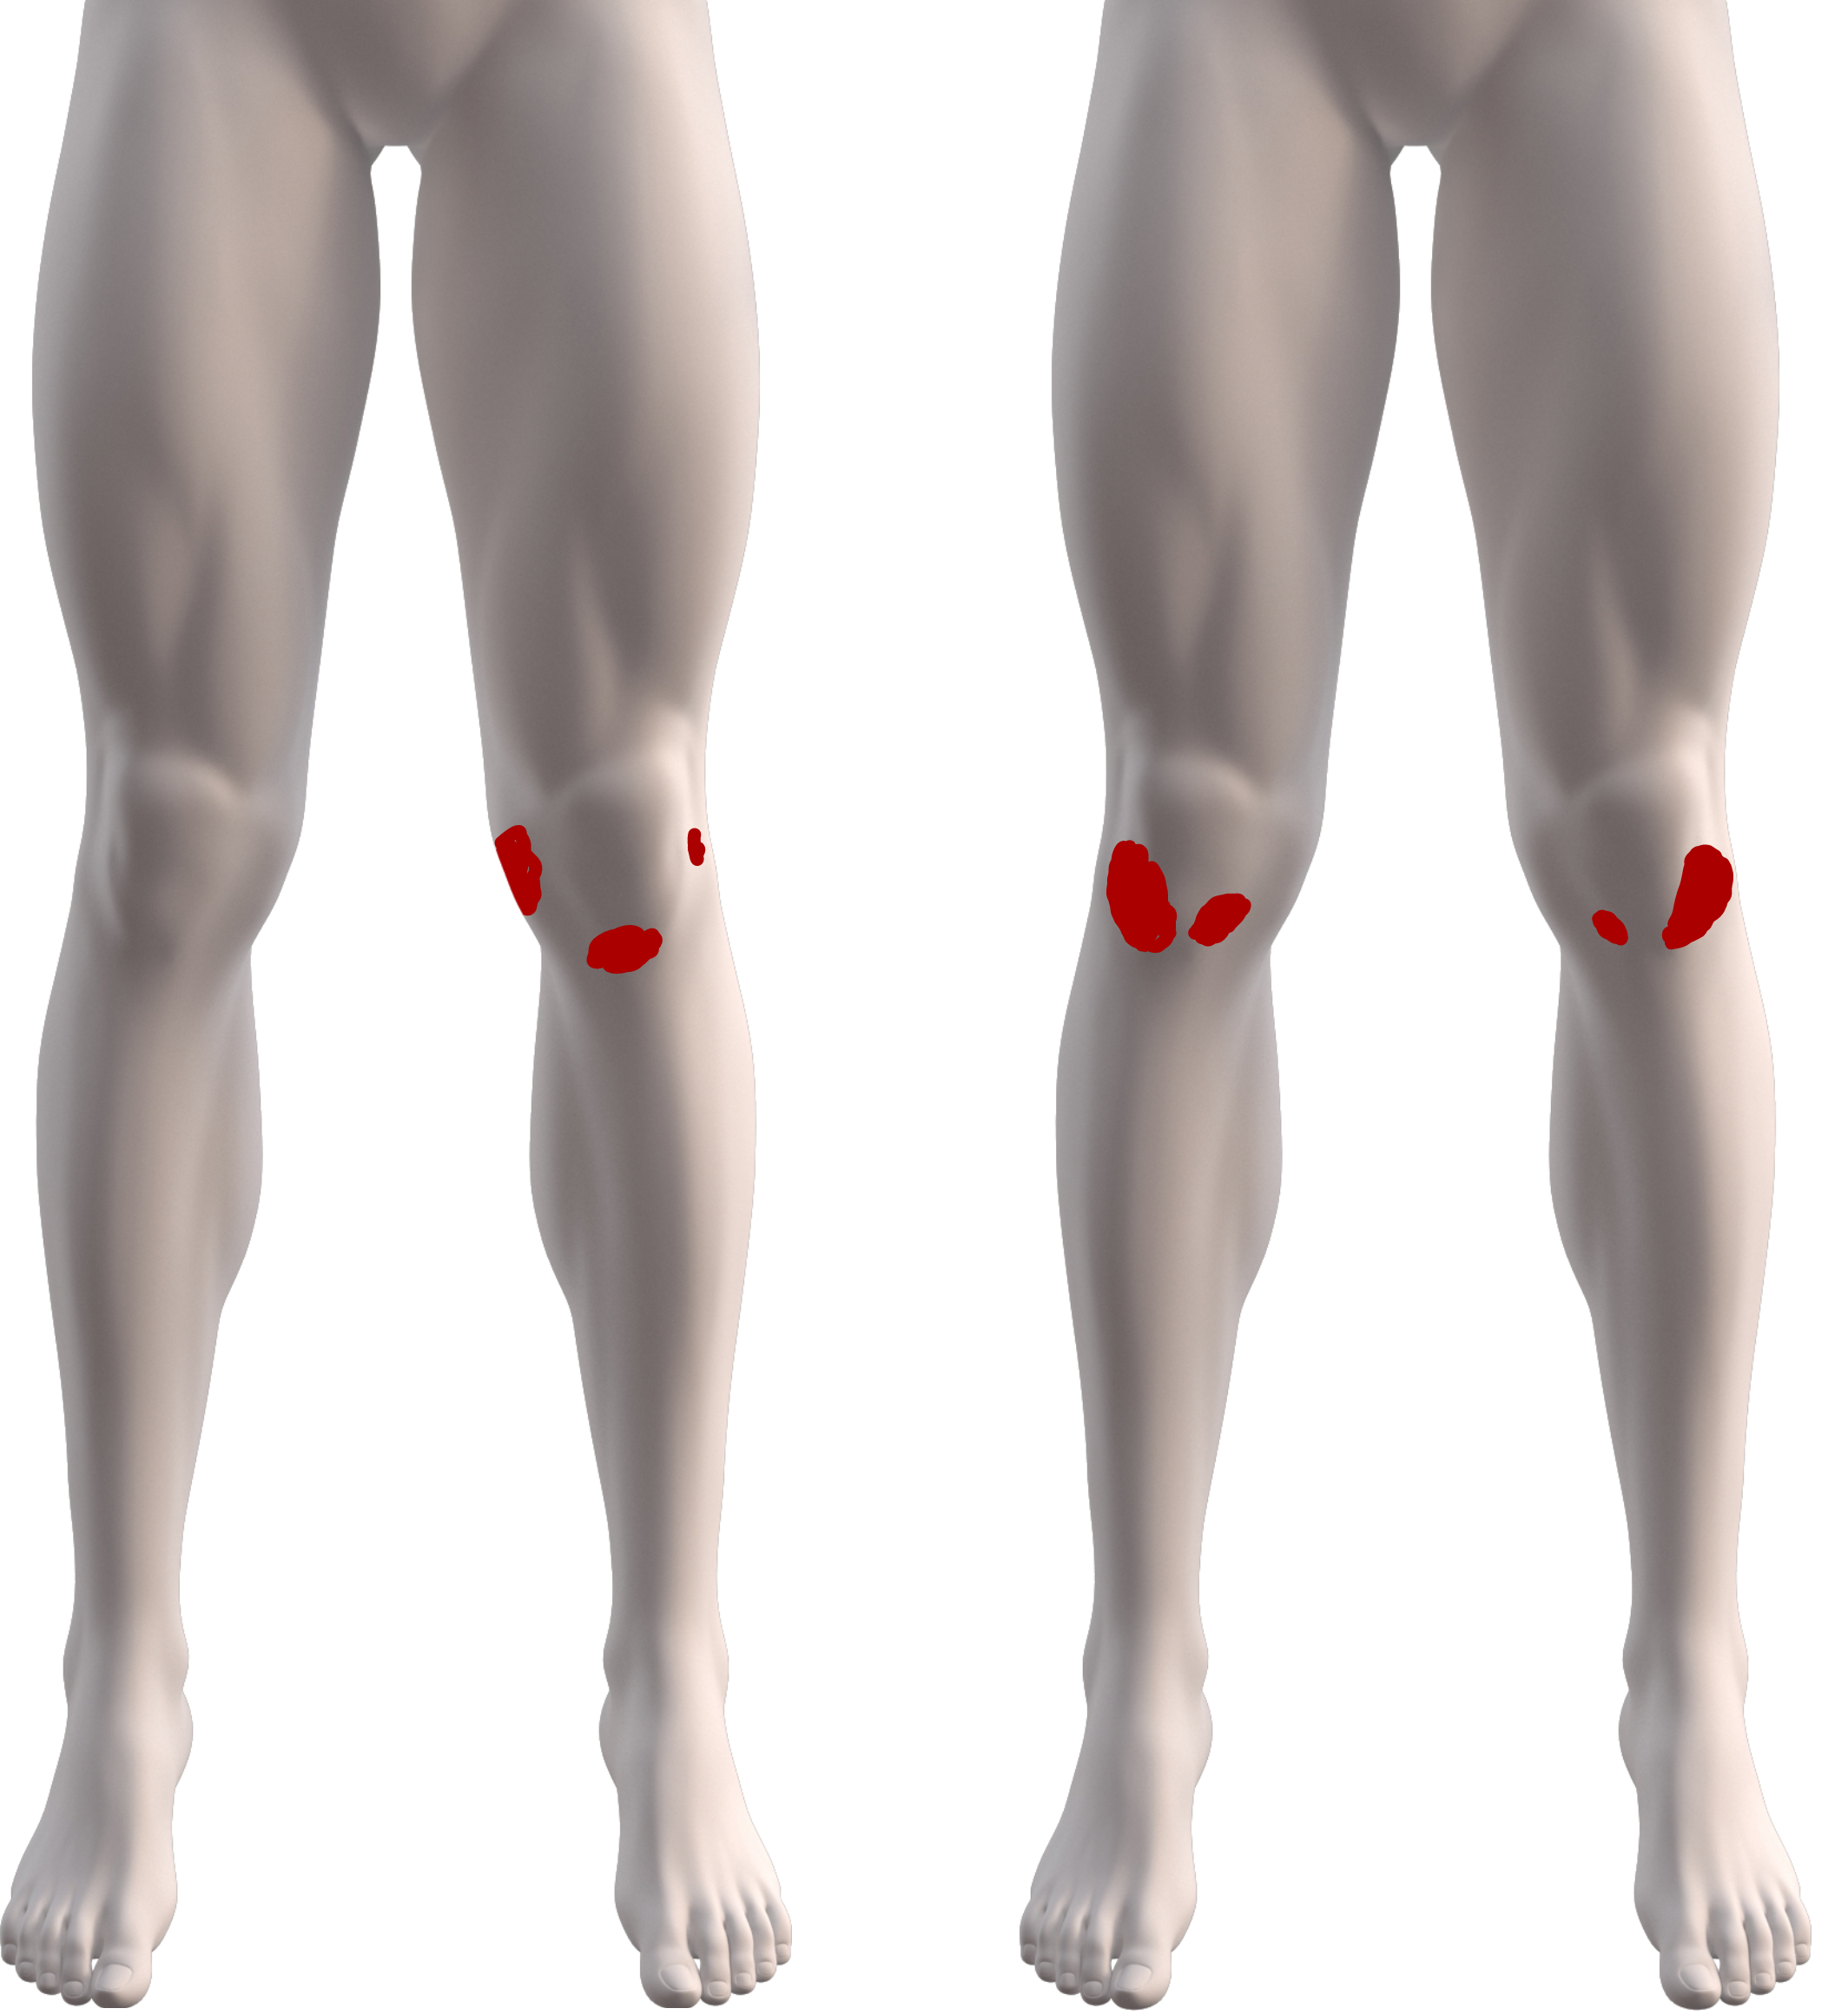
\includegraphics[width=0.35\textwidth]{Figures/twoPainmaps}
\caption{Pain maps from two individuals with uni- and bilateral PFP. The red markings indicate the area of pain perceived by the individuals.}
\label{fig:twoPainmaps}
\end{figure}

\noindent
The number of pain maps associated with pain duration was 205, and 197 associated with pain intensity measured according to the Visual Analog Scale (VAS).
In order to improve the performance of the deep learning models, gender was included as an additional input. This was chosen because females tend to report more intense and frequent pain than males \citep{Pieh2012}. 

\subsection{Pre-processing of pain maps}
The pain maps were processed in MatLab v. R2017b, where the images were resized, since they were collected with different resolutions (screen sizes) and cropped to only include the knees. To increase the amount of pain maps, a split body approach was chosen because deep learning models may benefit while using a larger dataset. Using the split body approach, the knees in the pain maps were separated into a single knee pain image. The left knee was then mirrored to resemble the right knee to minimize the variance in the images. The final pain maps had resolutions of $252 \times 118$ pixels.
By using split body approach it was assumed that the pain duration and pain intensity were identical for both knees if PFP was bilateral. This resulted in an increased total number of pain maps with gender and pain duration to 333, and pain maps with gender and pain intensity to 319. \newline
\noindent
The models were designed to classify pain maps according to pain duration or pain intensity divided into two classes with intervals based on the extremes. The classification intervals were 0 to 12 months and 36 to 300 months for pain duration, and 0 to 4 and 8 to 10 for pain intensity measured on VAS. The reason for choosing extreme intervals, was to separate closely related patterns between the two classes, which resulted in the number of pain maps as shown in Table \ref{tab:painmaps}.

\begin{table}[H]
\centering
\begin{tabular}{@{}lcccc@{}}
\toprule
   & \multicolumn{2}{c}{Pain duration (months)} & \multicolumn{2}{c}{Pain intensity (VAS)} \\ \midrule
   & 0-12                & 36-300               & 0-4                & 8-10                \\ \midrule
MR & 114                 & 122                  & 72                 & 124                 \\
LR & 105                 & 118                  & 68                 & 118                 \\
CR & 113                 & 121                  & 71                 & 123                 \\ \bottomrule
\end{tabular}
\caption{The number of pain maps for MR, LR, and CR for both pain duration and pain intensity using the extremes.}
\label{tab:painmaps}
\end{table}

\subsubsection{Morphology-representation (MR)}
The original pain maps reflect the morphology of the pain, which refers to its shape and distribution. The original pain maps were converted into binary matrices, where the pain was indicated with "1" and no pain as "0". This representation did not require further processing than converting the pain maps to a matrix including gender and the output, pain duration or pain intensity. 

\subsubsection{Location-representation (LR)} 
A simplified representation of the pain maps was created to investigate whether the location has patterns related to the pain duration or pain intensity. The location of the pain was reflected by the use of knee regions shown in Fig. \ref{fig:atlas}, where the regions are based on the underlying anatomical structures.
The location were divided into ten regions, which were inspired by Photographic Knee Pain Map (PKPM). The divisions were designed to categorize location of knee pain for diagnostic and research purposes.\citep{Elson2010}

\begin{figure} [H] 
\centering
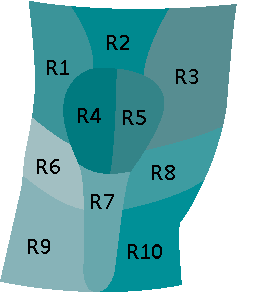
\includegraphics[width=0.22\textwidth]{Figures/atlas}
\caption{The regions of the right knee (R1-R10).}
\label{fig:atlas}
\end{figure}

\noindent 
There are ten regions, where regions 1 and 3 represent the superior lateral and superior medial areas for patella. Region 2 refers to quadriceps tendon. The patella is divided into lateral and medial regions, which are regions 4 and 5. Regions 6 and 8 are lateral and medial joint line areas. Patella's tendon is region 7 and the two last regions, 9 and 10, are tibia lateral and medial.\citep{Elson2010} \newline
\noindent
A vector consisting of ten elements was created, where each value represented either an active region (1) or a not active region (0). The values were defined by using a threshold to determine whether a region was considered active in relation to the amount of pain pixels in the specific region. The threshold was used to accommodate for the diffuse pain and the difficulty in localizing PFP. The threshold increased the confidence of an active pain region by avoiding minimal contributions. Simultaneously, the threshold should not be too high so too many or big areas were excluded. The threshold indicated which minimal percentage of pain pixels, that should be present in a specific region before it was considered as active. The threshold was decided based on an analysis of five random pain maps, where threshold values of 0, 5, 10 and 15\% were compared. Based on the analysis, a 5\% threshold was chosen.  

\subsubsection{Combined-representation (CR)}
A combination of morphology and location of the pain was created based on components from MR and LR. The original pain maps were superimposed on the knee regions, which resulted in pain pixels reflecting the location with a number from one to ten. Before using the representation as input in the deep learning models, a one-hot encoding approach was used, which made it possible to separate categorical data into binary data \citep{Harris2012}. As a result, the ten values did not have a relation to each other when analysed in the deep learning models. 


\begin{figure*} [t!]
%\begin{tcolorbox}[colframe=black!30!black, colback=white]
\centering
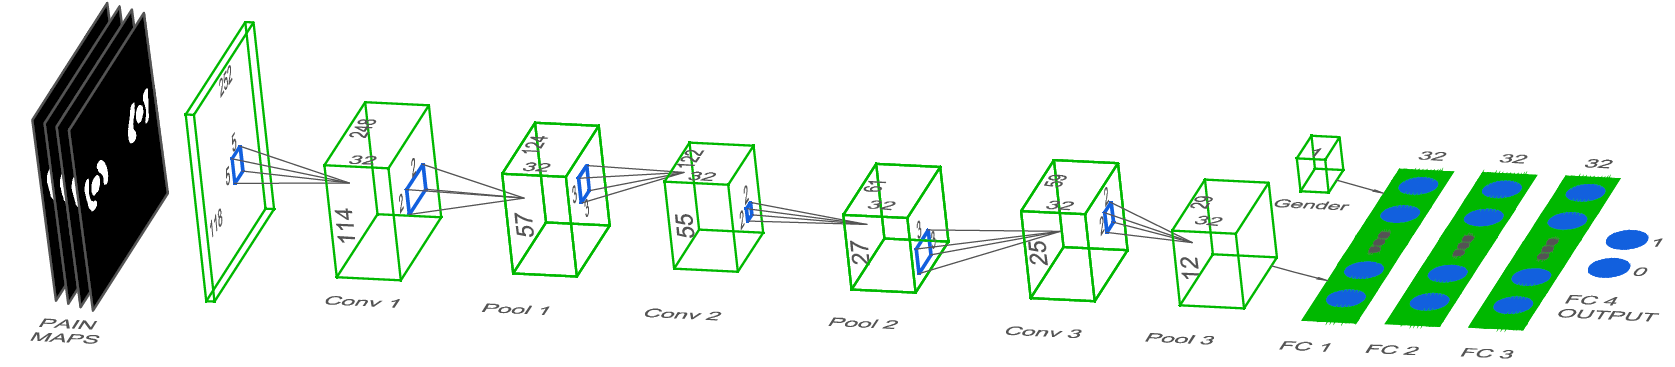
\includegraphics[width=1\textwidth]{Figures/models}
\caption{The architecture of the deep learning models including the MR before optimization. The models consisted of three convolutional, three max pooling, and four fully connected layers. The gender was included in the first fully connected layer. The boxes represent the output after each layer.}
\label{fig:models}
%\end{tcolorbox}
\end{figure*}

\subsection{Architecture of the deep learning models}
Deep learning models were developed on a computer with 4x "Intel® Core™ i7" CPUs and one single GPU of type "Geforce GTX 970M", using the programming language Python v3.6.3. Libraries used was Keras v2.0.8 with a TensorFlow v1.3.0 backend.\newline
\noindent
Six deep learning models for the three pain map representations and pain duration or pain intensity were created. The models used supervised learning, which is defined as a network learning to classify a given input corresponding to a specific output \citep{Goodfellow2016}. The models were designed differently according to each pain map representation and type of classification. The architecture of the models, before optimization, including the MR is illustrated in Fig. \ref{fig:models}. The models classified MR and CR consisted of three convolutional layers, to which a max pooling layer was added after each convolutional layer, and followed by four fully connected layers, where gender was inserted as a secondary input for the models. The only difference in the models using the CR was the input image, which was represented as a matrix with ten layers. 
The models including LR consisted of only four fully connected layers of the architecture shown in Fig. \ref{fig:models}. 

\subsubsection{The convolutional layers}
Convolutional Neural Networks (CNNs) is a type of neural network for processing data with a grid-like topology \citep{Goodfellow2016}. CNNs were used to classify MR and CR because of its capability to perform highly according to image classification. The purpose of the convolutional layers was to recognize features in the pain maps by taking the image and scan it, and then split it up into feature maps.\citep{Goodfellow2016,LeCun1998} The first convolutional layer consisted of a kernel size of $5 \times 5$ and 32 filters. The two following convolutional layers consisted of kernel sizes on $3 \times 3$ and 32 filters. 

\subsubsection{Max pooling layers}
For the models containing convolutional layers, each convolution layer was followed by a max pooling layer, which is a typical structure of a convolutional network \citep{Goodfellow2016, LeCun2015}.
Max pooling layers are used to reduce the size of the dataset, while maintaining features from the feature maps. Given a reduction in the data, the computation speed may increase.\citep{Goodfellow2016,LeCun1998} 
Max pooling layers were defined after each convolutional layer, to which all have a kernel size of $2 \times 2$ with a stride of 2. From the kernel window, the highest of the 4 values was extracted to next layer and used further through the network. 

\subsubsection{Fully connected layer and output layer}
All the models consisted of four fully connected layers, where the first layer received a flattened version of the input. The notation for gender was included in the end of the array, which was used as input in the first fully connected layer with 32 nodes. Additionally, the second and third layers consisted of 32 nodes. The fourth fully connected layer, which also was the output layer, included a sigmoid activation function. 
This function operates with a single output, that saturates when its input is either extremely negative or extremely positive \citep{Goodfellow2016}. The single output refers to the number of classification intervals, pain duration 0-12 month, and 36-300 months, or pain intensity 0-4, and 8-10 on VAS. 

\subsubsection{Rectified Linear Unit activation function}
The activation function, chosen for all hidden layers in the models, was Rectified Linear Unit (ReLU), which transforms the linear output to a nonlinear function by making all negative values to zero. The ReLU function still remains nearly linear, which means it can easily be optimized with gradient descent based methods. In modern neural networks, ReLU is recommended to use as a default activation function and could be defined as $g(x) = max\{0, x\}$.\citep{Goodfellow2016}

\subsubsection{Dropout algorithm}
A dropout algorithm was implemented for the models in the first two hidden fully connected layers to reduce overfitting while training. The algorithm works by randomly dropping a specified fraction of the nodes in the given layer, to which the nodes that drop, and changes between different nodes during the training \citep{Srivastava2014}. Dropout reduces the nodes’ ability for co-adaptation, where multiple nodes compute the same features. For the models, the dropout fraction was set to 0.5 (50\%) based on a previous study by \citeauthor{Srivastava2014} \citep{Srivastava2014}, which found 0.5 as optimal for multiple ranges of networks.

\subsubsection{Back-propagation algorithm}
Back-propagation was used for the learning process where the weights of the models were adjusted in order to reduce the error calculated between the predicted output, and the correct output \citep{Duda2000}. Back-propagation is based on gradient descents, which computes gradients from the output to the input, in order to minimize the overall output error as much as possible during the learning stage. 
After each pass of a minibatch, the inputs and weights were multiplied for each node summed with additional coefficient bias.\citep{LeCun1998, Hameed2016}
Afterwards, a loss was calculated based on a loss function for every input that passed through the network to make the adjustments on the parameters to reduce the loss. As training progressed, the loss should decrease as a result of the parameter updates, and improve the performance of the neural network.\citep{Goodfellow2016, LeCun2015, Duda2000} This learning process continued until optimal parameters with minimum error were reached.\citep{Hameed2016}

\vspace{-0.2cm}
\subsection{Training of the models}
The models were trained and optimized with a structured grid search of hyperparameters to help set the initial parameters for the models. These hyperparameters refer to learning rate, number of filters and nodes, and number of epochs with different batch sizes. Accuracy was used to determine the improvement of performance when testing the multiple parameters.
Further, the pain maps were divided into three subsets, a training set consisting of 75\%, a validation set consisting of 10\%, and a test set of the remaining 15\%. A manual optimization was performed, using the validation set, by evaluating the development in loss, accuracy during training, and the general performance estimated from accuracy. After optimization, the models were tested with the test set, using the hyperparameters from the optimization.
 
 
\subsection{Nonlinearity in pain maps} 
Additionally, linear regressions were made to validate whether the deep learning models used more than the simple features to predict either pain duration or pain intensity.
Given that PFP is subjective and multifactorial it is unlikely that the pain maps and pain intensity are linearly correlated. In order to determine if there was indeed a linear relationship, linear regressions were done on simple features reflecting the size of the pain and number of active pain regions. Linear regressions were made in MatLab, and composed correlations between; number of pain pixels and pain duration, number of pain pixels and pain intensity, number of active pain regions and pain duration, and number of active pain regions and pain intensity.

%\begin{figure*} [b!]
%\begin{tcolorbox}[colframe=black!30!black, colback=white]
%\centering
%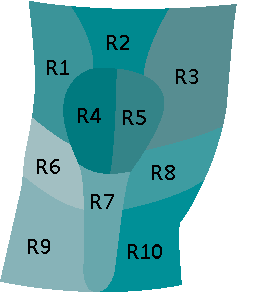
\includegraphics[width=0.2\textwidth]{Figures/atlas}
%\caption{SÅDAN LAVER VI EN BOXER MED ET BILLED}
%\label{fig:atlas1}
%\end{tcolorbox}
%\end{figure*}



%\begin{figure*} [b!]
%\begin{tcolorbox}[colframe=black!30!black, colback=white]
%  \begin{subfigure}[b]{0.45\textwidth}
%    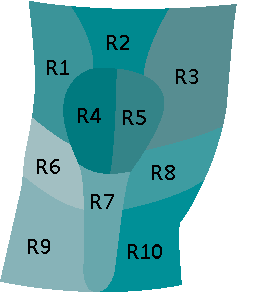
\includegraphics[width=\textwidth]{Figures/atlas}
%    \caption{FUCK JA}
%    \label{fig:f11}
%  \end{subfigure}
%  \hfill
%  \begin{subfigure}[b]{0.45\textwidth}
%    \includegraphics[width=\textwidth]{Figures/twopainmaps}
%    \caption{FUCK NEJ}
%    \label{fig:f22}
%  \end{subfigure}
%  \caption{SÅDAN SÆTTER VI TO BILLEDER I EN}
%\end{tcolorbox}
%\end{figure*}